%!TEX program = xelatex
\documentclass[11pt, a4paper]{article}
  \usepackage[a4paper,top=3cm,bottom=4cm,left=2.5cm,right=2.5cm]{geometry}
  \usepackage{subfig}
  \usepackage{graphicx}
  \graphicspath{{../images/}}
  \usepackage{hyperref}
  \usepackage{amsmath}
  \usepackage{braket}
  \usepackage{enumitem}
  \usepackage{multirow}
  \usepackage{mathtools}
  \usepackage{xepersian}
  \settextfont[Scale=1.2]{B Nazanin}
  \setlatintextfont[Scale=1]{Times New Roman Cyr}
  \title{\textbf{شبیه‌سازی رایانه‌ای در فیزیک}\\تمرین هشتم: انتگرال تعینی}
  \author{سینا معمر ۹۵۱۰۲۳۱۶}
    

\begin{document}

\maketitle
\thispagestyle{empty}


\section{\textbf{معادله دیفرانسیل مرتبه اول}}
کد این بخش از تمرین را در فایل
\lr{q1.py}
می‌توان مشاهده نمود.
ابتدا قبل از حل عددی معادله،
باید آن را به یک معادله بی‌بعد تبدیل کنیم تا اثر واحد‌ها از بین برود و با عدد‌های خیلی کوچک و یا بزرگ مواجه نشویم.
برای بی‌بعد کردن معادله به صورت زیر عمل می‌کنیم:

\begin{equation}
  R \frac{dQ}{dt} + \frac{Q}{C} = V
  \Rightarrow
  \frac{RC}{VC} \frac{dQ}{dt} + \frac{Q}{VC} = 1
\end{equation}

\begin{equation}
  \begin{cases}
    Q^{'} = \frac{Q}{VC} \\
    \tau = \frac{t}{RC}
  \end{cases}
  \Rightarrow
  \frac{dQ{'}}{d\tau} + Q^{'} = 1
  \label{eqn:q1_nondim_eqn}
\end{equation}
معادله‌ی بالا یک معادله‌ی بی‌بعد است که در نتیجه دوره تناوب آن از مرتبه‌ی
$1$
است.
با توجه به مقادیر داده شده خواهیم داشت:

\begin{equation}
  \begin{cases}
    Q^{'} = Q \times 10^5 \\
    \tau = \frac{t}{3} \times 10^3
  \end{cases}
\end{equation}

شبیه‌سازی را برای زمان
$t = 21 \text{\lr{ ms}}$
یا معادلا
$\tau = 7$
با قدم‌های
$h = 10^{-4}$
انجام می‌دهیم.
نتیجه‌ی به دست آمده را در شکل
\ref{fig:q1_euler_analytic}
می‌توان مشاهده نمود.
همان‌طور که دیده می‌شود جواب به دست آمده به خوبی با جواب تحلیلی تطابق دارد.
برای مشاهده‌ی رابطه‌ی خطای جواب نهایی با مقدار
$h$،
باید برای
$h$
های مختلف مقدار نهایی را با استفاده از روش اویلر به دست آورد و سپس خطای نسبی آن را رسم نمود.
نمودار به دست آمده را در شکل
\ref{fig:q1_euler_error}
می‌توان مشاهده نمود.
همان‌طور که انتظار داشتیم نمودار تمام لگاریتم آن خطی با شیب
$0.997 \approx 1$
است.
در نتیجه
$\Delta Q / Q = O(h)$
خواهد بود که با تئوری نیز هم‌خوانی دارد.

\begin{figure}[h!]
	\centering
  \begin{minipage}[b]{0.48\textwidth}
    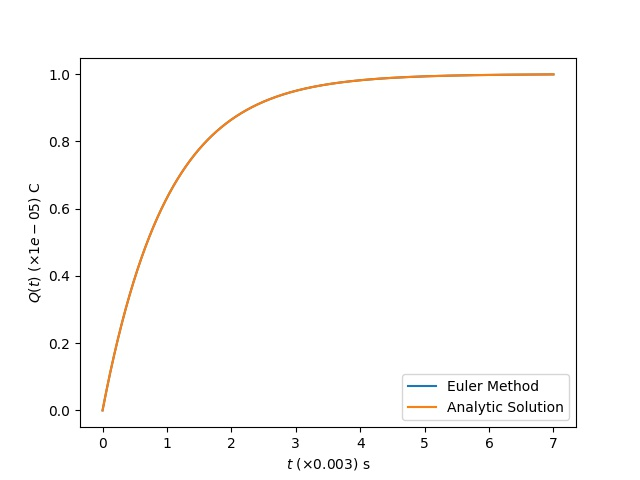
\includegraphics[width=\textwidth]{q1_euler_analytic_0_7.0_0.0001.jpg}
    \caption{مقایسه‌ی جواب تحلیلی و جواب به دست آمده از روش اویلر برای معادله‌ی شارژ خازن با قدم‌های $h = 10^{-4}$}
    \label{fig:q1_euler_analytic}
  \end{minipage}
  \hfill
  \begin{minipage}[b]{0.48\textwidth}
    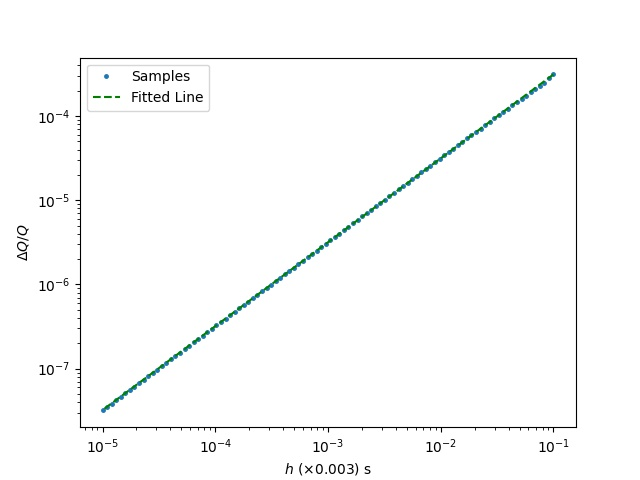
\includegraphics[width=\textwidth]{q1_euler_error_0.1_1e-05_100_7.0.jpg}
    \caption{خطای نسبی جواب نهایی به دست آمده از روش اویلر برای معادله‌ی شارژ خازن در زمان $t = 21 \text{\lr{ ms}}$ برای $h$ های مختلف}
    \label{fig:q1_euler_error}
  \end{minipage}
\end{figure}


\section{\textbf{معادله دیفرانسیل مرتبه دوم}}
کد این بخش از تمرین را در فایل
\lr{q2.py}
می‌توان مشاهده نمود.
معادله‌ی داده شده خود به صورت بی‌بعد است به همین دلیل نیازی برای تغییر دادن آن قبل از شبیه‌سازی نیست.
شبیه‌سازی را با استفاده از الگوریتم‌های گفته شده برای
$10$
برابر دوره تناوب جواب
$(t = 20\pi)$
و شرایط اولیه‌ی
$x_0 = 1$
و
$v_0 = 0$
انجام می‌دهیم.
نتیجه به دست آمده را در شکل
\ref{fig:q2_x_t}
می‌توان مشاهده نمود.
همان‌طور که دیده می‌شود جواب به دست آمده از روش های مختلف به جز روش اویلر،
به خوبی با جواب تحلیلی تطابق دارند.
ولی در مورد روش اویلر مشاهده می‌شود که با گذشت زمان،
دامنه‌ی نوسان افزایش می‌یابد و یا به عبارت دیگر انرژی سیستم پایسته نیست و افزایش می‌یابد.
هم‌چنین نمودار فضای فاز به دست آمده از روش‌های مختلف را در شکل‌های
\ref{fig:q2_euler}
تا
\ref{fig:q2_beeman}
می‌توان مشاهده نمود.
همان‌طور که دیده می‌شود در تمام ‌آن‌ها به جز روش اویلر،
نمودار فضای فاز به صورت دایره‌ است که نشان‌دهنده‌ی پایستگی انرژی در معادله می‌باشد.
ولی در نمودار به دست آمده از روش اویلر شاهد هستیم که شعاع دایره به تدریج افزایش می‌یابد و
به عبارت دیگر انرژی زیاد می‌شود که این بر خلاف ذات معادله است.
پس برای این معادله تمامی‌ روش‌ها به جز اویلر پایستگی انرژی را حفظ می‌کنند.

\begin{figure}
  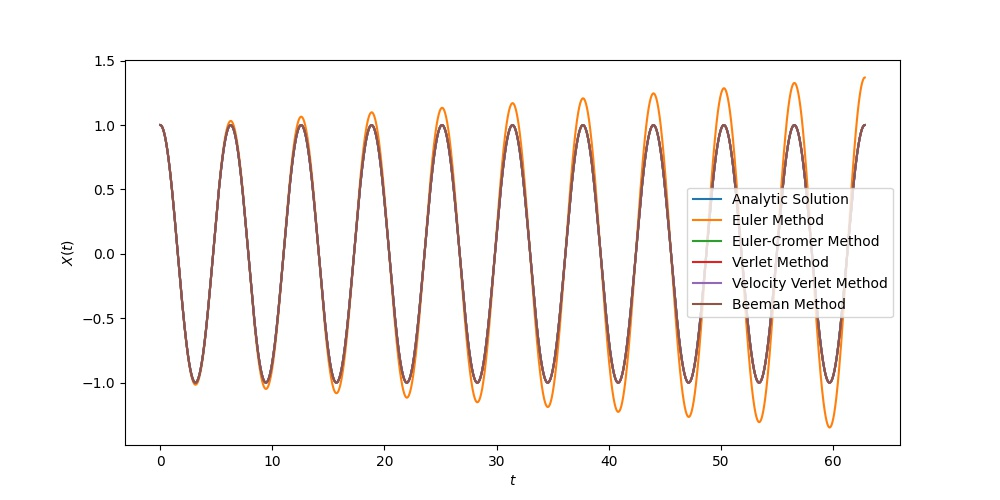
\includegraphics[width=\textwidth]{q2_x_t_0_62.83185307179586_0.01_[1, 0].jpg}
  \caption{مقایسه‌ی نمودار مکان بر حسب زمان به دست آمده برای معادله‌ی داده شده با استفاده از الگوریتم‌های مختلف با جواب تحلیلی برای $h = 10^{-2}$ و شرایط اولیه‌ی $x_0 = 1$ و $v_0 = 0$}
  \label{fig:q2_x_t}
\end{figure}

\begin{figure}[h!]
	\centering
  \begin{minipage}[b]{0.4\textwidth}
    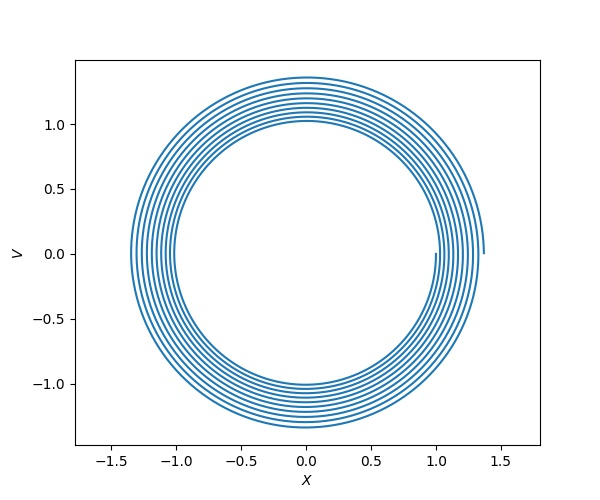
\includegraphics[width=\textwidth]{q2_v_x_Euler Method_0_62.83185307179586_0.01_[1, 0].jpg}
    \caption{نمودار تغییرات سرعت بر حسب مکان برای معادله‌ی داده شده و با روش اویلر و با قدم‌های $h = 10^{-2}$ و با $x_0 = 1$ و $v_0 = 0$}
    \label{fig:q2_euler}
  \end{minipage}
  \hfill
  \begin{minipage}[b]{0.4\textwidth}
    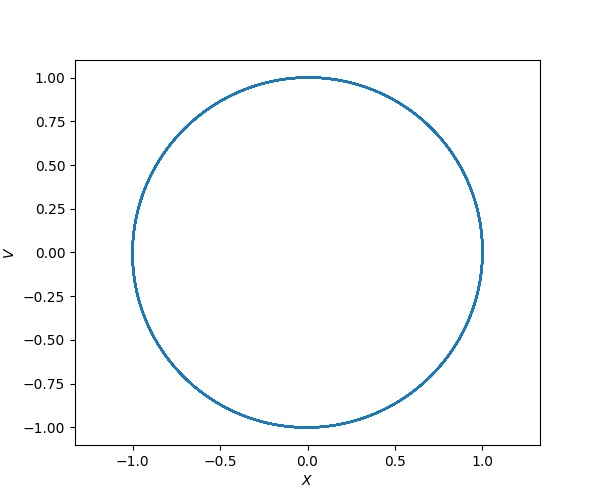
\includegraphics[width=\textwidth]{q2_v_x_Euler-Cromer Method_0_62.83185307179586_0.01_[1, 0].jpg}
    \caption{نمودار تغییرات سرعت بر حسب مکان برای معادله‌ی داده شده و با روش اویلر-کرامر و با قدم‌های $h = 10^{-2}$ و با $x_0 = 1$ و $v_0 = 0$}
    \label{fig:q2_euler_cromer}
  \end{minipage}
  \begin{minipage}[b]{0.4\textwidth}
    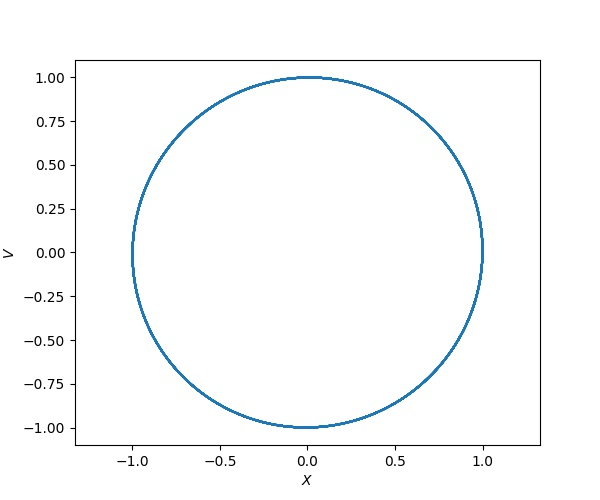
\includegraphics[width=\textwidth]{q2_v_x_Verlet Method_0_62.83185307179586_0.01_[1, 0].jpg}
    \caption{نمودار تغییرات سرعت بر حسب مکان برای معادله‌ی داده شده و با روش ورله و با قدم‌های $h = 10^{-2}$ و با $x_0 = 1$ و $v_0 = 0$}
    \label{fig:q2_verlet}
  \end{minipage}
  \hfill
  \begin{minipage}[b]{0.4\textwidth}
    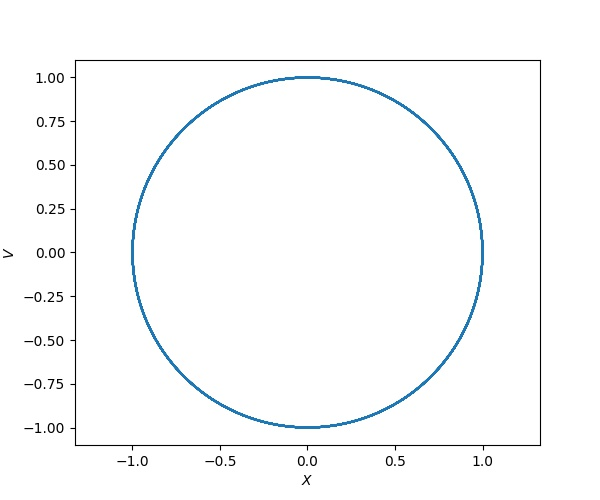
\includegraphics[width=\textwidth]{q2_v_x_Velocity Verlet Method_0_62.83185307179586_0.01_[1, 0].jpg}
    \caption{نمودار تغییرات سرعت بر حسب مکان برای معادله‌ی داده شده و با روش ورله سرعتی و با قدم‌های $h = 10^{-2}$ و با $x_0 = 1$ و $v_0 = 0$}
    \label{fig:q2_velocity_verlet}
  \end{minipage}
  \begin{minipage}[b]{0.4\textwidth}
    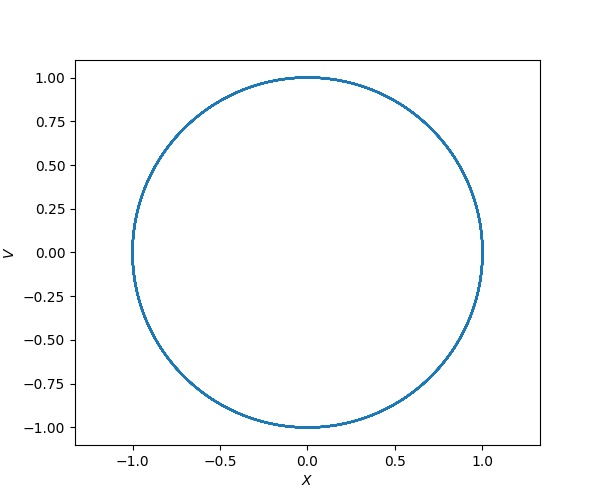
\includegraphics[width=\textwidth]{q2_v_x_Beeman Method_0_62.83185307179586_0.01_[1, 0].jpg}
    \caption{نمودار تغییرات سرعت بر حسب مکان برای معادله‌ی داده شده و با روش بیمن و با قدم‌های $h = 10^{-2}$ و با $x_0 = 1$ و $v_0 = 0$}
    \label{fig:q2_beeman}
  \end{minipage}
\end{figure}


\section{\textbf{ناپایداری الگوریتم‌ها}}
کد این بخش از تمرین را در فایل
\lr{q3.py}
می‌توان مشاهده نمود.
در این سوال معادله‌ی
\eqref{eqn:q1_nondim_eqn}
را با استفاده از الگوریتم داده شده حل عددی می‌کنیم.
نتیجه به دست آمده را در شکل
\ref{fig:q3_q_t}
می‌توان مشاهده نمود.
همان‌طور که دیده می‌شود جواب به دست آمده از حل عددی حول جواب تحلیلی نوسان می‌کند و دامنه‌ی این نوسان با گذشت زمان افزایش می‌یابد.
علاوه بر آن همان‌طور که دیده می‌شود 
با افزایش طول قدم‌ها یا معادلا کاهش دقت،
دامنه‌ی این نوسانات نیز افزایش می‌یابد.
در نتیجه با توجه به این رفتار،
پاسخ به دست آمده از این الگوریتم برای معادله‌ی شارژ خازن پایداری نخواهد داشت.

\begin{figure}
  \centering
  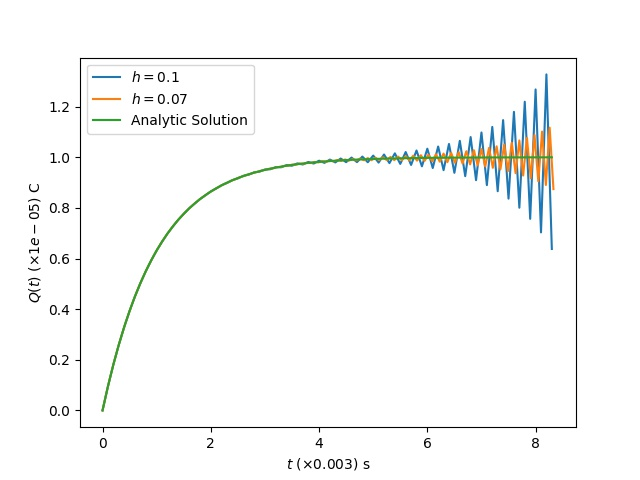
\includegraphics[width=.7\textwidth]{q3_0_8.333333333333334.jpg}
  \caption{حل معادله‌ی شارژ خازن با استفاده از الگوریتم داده شده برای $h = 0.1$ و $h = 0.07$ و مقایسه‌ی‌ آن‌ها با جواب تحلیلی}
  \label{fig:q3_q_t}
\end{figure}


\section{\textbf{آشوب}}
کد این بخش از تمرین را در فایل‌
\lr{q4.py}
می‌توان مشاهده نمود.
برای به دست‌آوردن مقادیر تناوبی
$x$
در هر
$r$،
تعدادی نقطه به طور تصادفی از بازه‌ی
$[0, 1)$
انتخاب می‌کنیم.
سپس این نقاط را به عنوان
$x_0$
در نظر می‌گیریم و با استفاده از معادله بازگشتی داده شده
$x_n$
را به دست می‌آوریم.
$n$
را باید به گونه‌ای انتخاب کنیم که جواب‌های به دست آمده به جواب‌های تناوبی نزدیک شده باشند.
نتیجه‌ی به دست آمده را در شکل
\ref{fig:q4_bifurcation_0_1}
می‌توان مشاهده نمود.
\\
برای به دست آودن مقادیر
$r_N$،
در نمودار به دست آمده زوم می‌کنیم و در آن‌ ناحیه با قدم‌های کوچک‌تر و با
$n$
بیش‌تر محاسبات را انجام می‌دهیم تا با دقت بیش‌تر بتوانیم این مقادیر را تعیین کنیم.
با دقت
$10^{-6}$
نهایتا تا
$N = 5$
می‌توانیم مقادیر را به دست بیاوریم.
نمودارهای به دست آمده را در شکل‌های
\ref{fig:q4_r_0}‌
تا
\ref{fig:q4_r_infty}
می‌توان مشاهده نمود.
با توجه به این نمودارها خواهیم داشت:

\begin{equation}
  \begin{cases}
    r_0 = 0.250000 \pm 10^{-6} \\
    r_1 = 0.749999 \pm 10^{-6} \\
    r_2 = 0.862372 \pm 10^{-6} \\
    r_3 = 0.886020 \pm 10^{-6} \\
    r_4 = 0.891101 \pm 10^{-6} \\
    r_5 = 0.892189 \pm 10^{-6} \\
    r_\infty = 0.892487 \pm 10^{-6}
  \end{cases}
\end{equation}
\\
برای محاسبه‌ی
$\delta$
لازم است که فاصله‌ی بین نقاط دوشاخگی را در حد
$n \rightarrow \infty$
داشته باشیم.
ولی از ‌آن‌جایی که برای محاسبه‌ی عددی این کار ناممکن است، باید تا حد ممکن برای
$n$
های بزرگ‌ این مقادیر را محاسبه کنیم.
علاوه بر این سختی دیگر این است که فاصله‌ی بین
$r_n$
ها به صورت هندسی کاهش می‌یابد،
در نتیجه برای محاسبه‌ی دقیق‌تر آن باید
$r_n$
ها را با دقت بسیار بیش‌تری تعیین نمود.
با دقت
$\Delta r = 10^{-6}$
می‌توان حداکثر
$r_n$
های قابل مشاهده در شکل‌های
\ref{fig:q4_r_3}
تا
\ref{fig:q4_r_5}
را به دست آورد.
با توجه به این نمودار‌ها خواهیم داشت:

\begin{equation}
  \delta \approx \frac{r_4 - r_3}{r_5 - r_4} = 4.668
\end{equation}
\\
برای محاسبه‌ی
$\alpha$
لازم است که خط
$x_m = 0.5$
را رسم کرده و محل تلاقی آن با نمودار را پیدا کنیم.
سپس در این نقاط اندازه‌ی دهانه‌ی دوشاخگی را به دست بیاوریم.
ولی باید توجه داشت که نسبت اندازه‌ی دو دهانه‌ی متوالی در حد
$n \rightarrow \infty$
برابر با مقدار دقیق
$\alpha$
خواهد شد.
ولی از طرف دیگر اندازه‌ی دهانه‌ها به صورت هندسی کاهش می‌یابد.
به همین دلیل نیاز است تا با دقت ‌بیش‌تری آن‌ها را محاسبه نمود.
با دقت
$\Delta r = 10^{-6}$
محل برخورد خط
$x_m$
با نمودار را برای
$R_3$
و
$R_4$
مطابق شکل‌های
\ref{fig:q4_R_3}
و
\ref{fig:q4_R_4}
به دست می‌آوریم.
با توجه به نمودار‌های به دست آمده خواهیم داشت:

\begin{equation}
  \begin{cases}
    R_3 = 0.888660 \pm 10^{-6}\\
    R_4 = 0.891667 \pm 10^{-6}
  \end{cases}
\end{equation}

حال باید مقدار نمودار در نزدیک‌ترین شاخه به
$x_m$
را در این نقاط به دست آورده و اندازه‌ی دهانه را حساب کنیم.
مقادیر به دست آمده به صورت زیر هستند:

\begin{equation}
  \begin{cases}
    d_3 = +0.04597432 \pm 10^{-8}\\
    d_4 = -0.01833121 \pm 10^{-8}
  \end{cases}
\end{equation}

\begin{equation}
  \Rightarrow
  \alpha \approx \frac{d_3}{d_4} = -2.508
\end{equation}



\begin{figure}
  \centering
  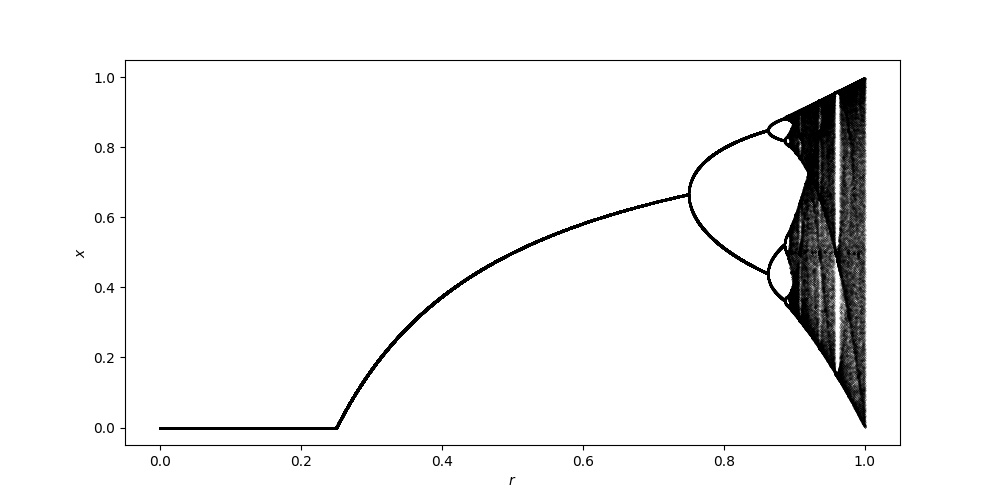
\includegraphics[width=.9\textwidth]{q4_0_1_10000_100_10000.jpg}
  \caption{نمودار دوشاخگی برای معادله لاجستیک برای $r \in [0, 1]$ با قدم‌های $\Delta r = 10^{-4}$ و با $100$ نمونه $x$ برای هر $r$ و محاسبه تا $n = 10^4$}
  \label{fig:q4_bifurcation_0_1}
\end{figure}

\begin{figure}[h!]
  \centering
  \begin{minipage}[b]{0.42\textwidth}
    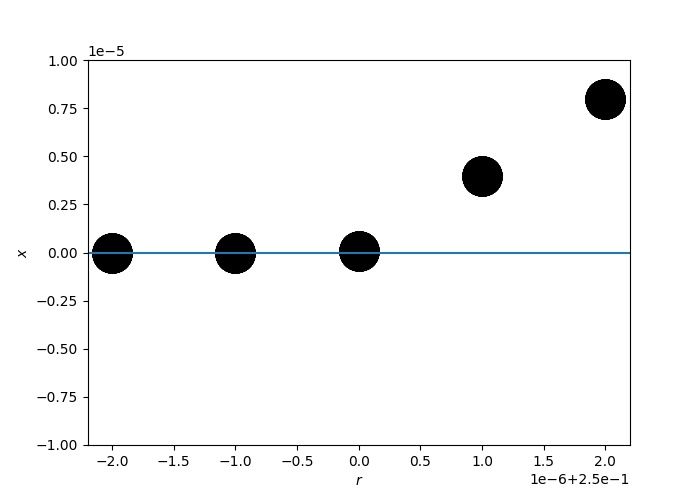
\includegraphics[width=\textwidth]{q4_0.249998_0.250002_5_10_10000000.jpg}
    \caption{نمودار دوشاخگی برای معادله لاجستیک حول $r_0$ با قدم‌های $\Delta r = 10^{-6}$ و با $100$ نمونه $x$ برای هر $r$ و محاسبه تا $n = 10^7$}
    \label{fig:q4_r_0}
  \end{minipage}
  \hfill
  \begin{minipage}[b]{0.42\textwidth}
    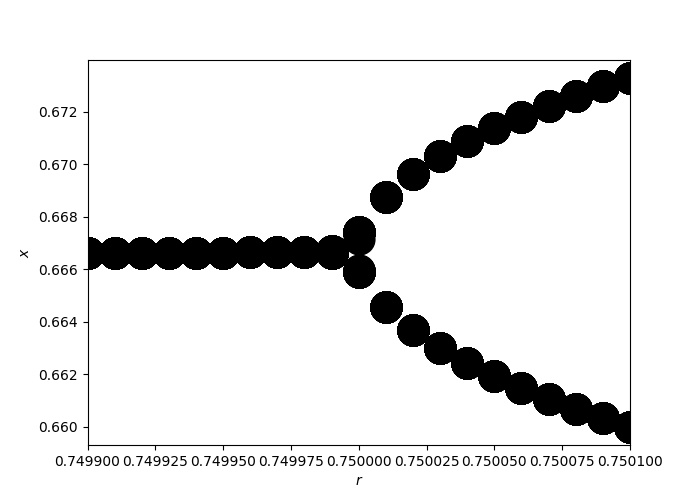
\includegraphics[width=\textwidth]{q4_0.7499_0.7501_21_100_100000.jpg}
    \caption{نمودار دوشاخگی برای معادله لاجستیک حول $r_1$ با قدم‌های $\Delta r = 10^{-6}$ و با $100$ نمونه $x$ برای هر $r$ و محاسبه تا $n = 10^5$}
    \label{fig:q4_r_1}
  \end{minipage}
  \begin{minipage}[b]{0.42\textwidth}
    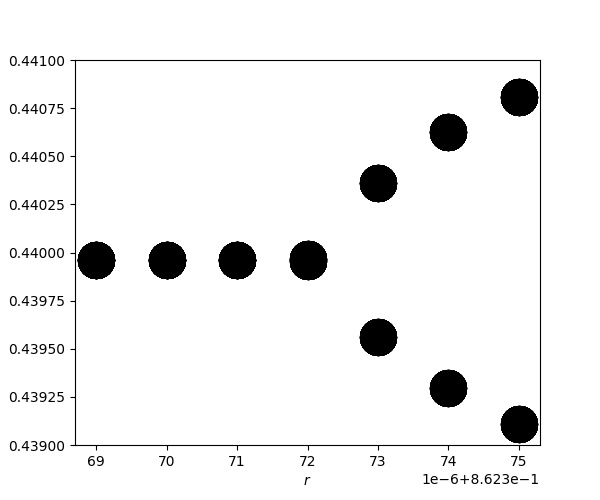
\includegraphics[width=\textwidth]{q4_0.862369_0.862375_7_100_1000000.jpg}
    \caption{نمودار دوشاخگی برای معادله لاجستیک حول $r_2$ با قدم‌های $\Delta r = 10^{-6}$ و با $100$ نمونه $x$ برای هر $r$ و محاسبه تا $n = 10^6$}
    \label{fig:q4_r_2}
  \end{minipage}
  \hfill
  \begin{minipage}[b]{0.42\textwidth}
    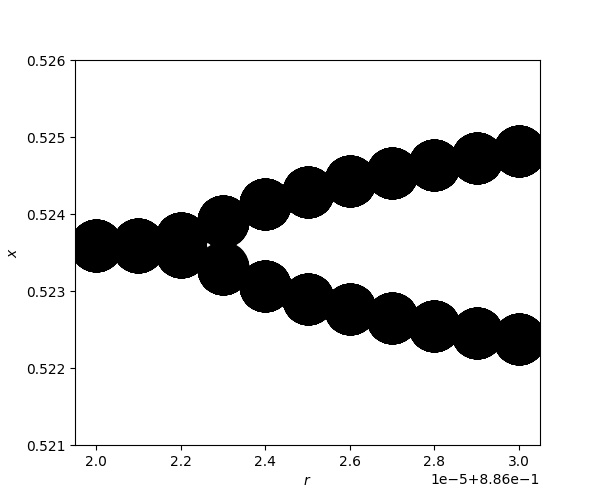
\includegraphics[width=\textwidth]{q4_0.88602_0.88603_11_100_100000.jpg}
    \caption{نمودار دوشاخگی برای معادله لاجستیک حول $r_3$ با قدم‌های $\Delta r = 10^{-6}$ و با $100$ نمونه $x$ برای هر $r$ و محاسبه تا $n = 10^5$}
    \label{fig:q4_r_3}
  \end{minipage}
  \begin{minipage}[b]{0.42\textwidth}
    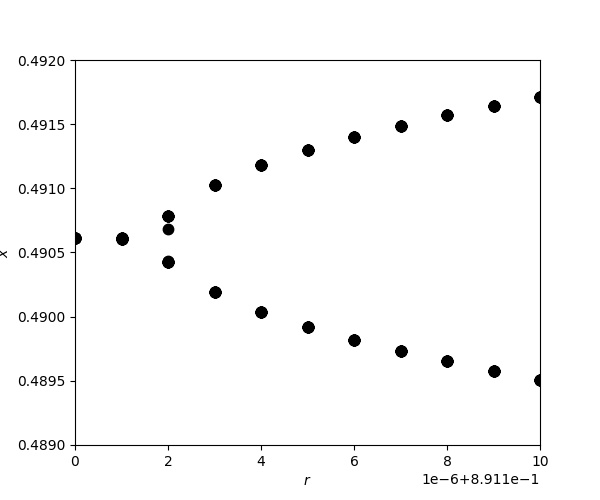
\includegraphics[width=\textwidth]{q4_0.8911_0.89111_201_100_100000.jpg}
    \caption{نمودار دوشاخگی برای معادله لاجستیک حول $r_4$ با قدم‌های $\Delta r = 10^{-6}$ و با $100$ نمونه $x$ برای هر $r$ و محاسبه تا $n = 10^5$}
    \label{fig:q4_r_4}
  \end{minipage}
  \hfill
  \begin{minipage}[b]{0.42\textwidth}
    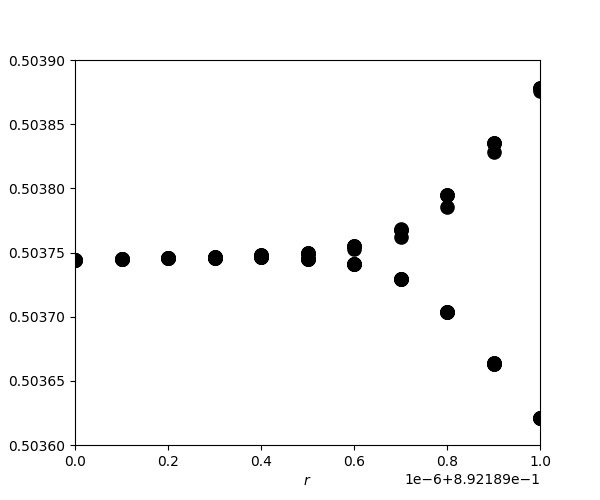
\includegraphics[width=\textwidth]{q4_0.892189_0.89219_21_100_100000.jpg}
    \caption{نمودار دوشاخگی برای معادله لاجستیک حول $r_5$ با قدم‌های $\Delta r = 10^{-6}$ و با $100$ نمونه $x$ برای هر $r$ و محاسبه تا $n = 10^5$}
    \label{fig:q4_r_5}
  \end{minipage}
\end{figure}

\begin{figure}[h!]
	\centering
  \begin{minipage}[b]{0.42\textwidth}
    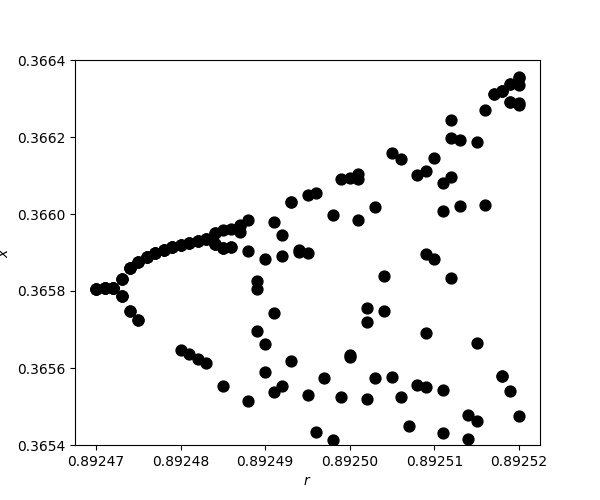
\includegraphics[width=\textwidth]{q4_0.89247_0.89252_51_100_100000.jpg}
    \caption{نمودار دوشاخگی برای معادله لاجستیک حول $r_\infty$ با قدم‌های $\Delta r = 10^{-6}$ و با $100$ نمونه $x$ برای هر $r$ و محاسبه تا $n = 10^5$}
    \label{fig:q4_r_infty}
  \end{minipage}
\end{figure}

\begin{figure}[h!]
	\centering
  \begin{minipage}[b]{0.48\textwidth}
    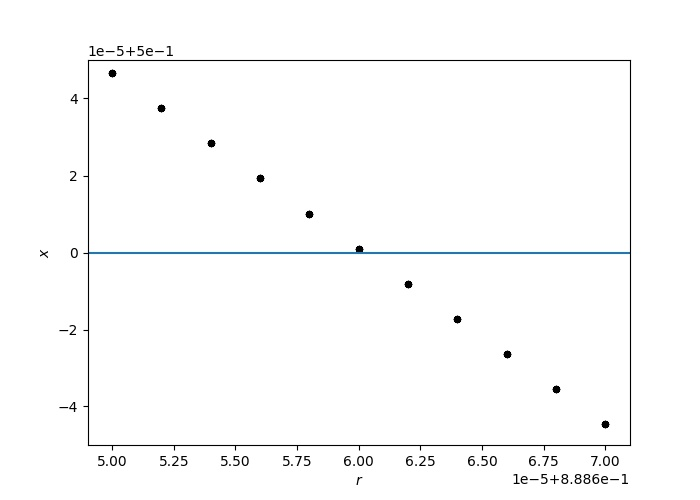
\includegraphics[width=\textwidth]{q4_0.88865_0.88867_11_100_100000.jpg}
    \caption{نمودار دوشاخگی و خط $x_m$ برای معادله لاجستیک حول $R_3$ با قدم‌های $\Delta r = 10^{-6}$ و با $100$ نمونه $x$ برای هر $r$ و محاسبه تا $n = 10^5$}
    \label{fig:q4_R_3}
  \end{minipage}
  \hfill
  \begin{minipage}[b]{0.48\textwidth}
    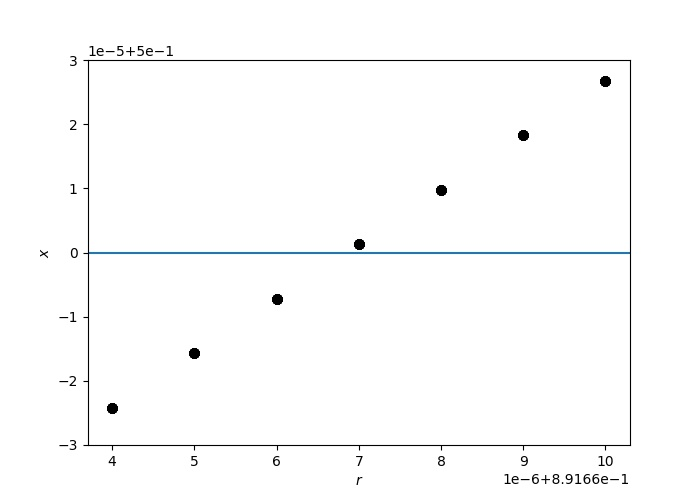
\includegraphics[width=\textwidth]{q4_0.891664_0.89167_7_100_10000.jpg}
    \caption{نمودار دوشاخگی و خط $x_m$ برای معادله لاجستیک حول $R_4$ با قدم‌های $\Delta r = 10^{-6}$ و با $100$ نمونه $x$ برای هر $r$ و محاسبه تا $n = 10^5$}
    \label{fig:q4_R_4}
  \end{minipage}
\end{figure}


\begin{equation}
  p = A e^{+k_{\text{\lr{real}}}x} e^{jwt}
\end{equation}


\end{document}
